%% SOICT 2026 submission -- Springer CCIS, which uses the LNCS class (llncs.cls).
%% Conference rules enforced below:
%%   - 12 pages excluding references
%%   - single-blind, so author names and affiliations ARE included
%%   - "submissions ... should not include page numbers"  -> \pagestyle{empty}
%% Build: Overleaf, pdfLaTeX. Stock llncs.cls, no layout overrides.
%% CAMERA-READY: delete the two \pagestyle/\thispagestyle{empty} lines to restore
%% Springer's running heads and folios.

\documentclass[runningheads,a4paper]{llncs}

\usepackage[T1]{fontenc}
\usepackage[utf8]{inputenc}
\usepackage{amsmath}
\usepackage{amssymb}
\usepackage{booktabs}
\usepackage{graphicx}
\usepackage{tikz}
\usepackage{array}
\usepackage[hidelinks]{hyperref}

\newcommand{\rulename}[1]{\textsc{#1}}
\setlength{\emergencystretch}{1.5em}  % break long cite/number lines instead of overflowing

\begin{document}
\pagestyle{empty}          % SOICT 2026: no page numbers anywhere in the submission PDF

\title{Separating the Action Gate from Geometry in\\ Execution-Based Evaluation for GUI Instruction Generation}

\titlerunning{Separating the Action Gate from Geometry}

\author{Le Doan Phuong Uyen\inst{1} \and Nguyen Hong Buu Long\inst{1}}

\authorrunning{L. D. P. Uyen and N. H. B. Long}

\institute{Faculty of Information Technology, University of Science, VNU-HCM,\\
Ho Chi Minh City, Vietnam\\
\email{24C15039@student.hcmus.edu.vn}, \email{nhblong@fit.hcmus.edu.vn}}

\maketitle
\thispagestyle{empty}      % \maketitle resets the first page to "plain"; undo that

\begin{abstract}
Instruction generation for graphical user interfaces cannot be evaluated by string overlap
against a single reference, since many wordings identify the same widget. Evaluation is instead
execution-based: an independent grounding model reads the generated sentence,
predicts a point on the screenshot, and the sentence is counted correct when that point matches
the recorded touch under a matching rule taken from the GUI-agent literature. We study this matching rule. Every rule in current use conjoins an
\emph{action-type gate} with a \emph{geometric} predicate, including AndroidControl's
Appendix D.3 predicate, both variants of the Android-in-the-Wild matcher, and the fixed
tolerance windows between them. As the tolerance is relaxed, the score therefore measures
less of the localisation and more of the gate. On $4{,}463$ AndroidControl touch steps we place seven such
rules on a single strictness ladder, bounded by the geometric predicate alone and the gate alone. For one fixed pair of
systems, the measured difference is $+0.41$ points under the rule that carries no gate
(95\% CI covering zero) and $+4.39$ under the gate alone, with the seven coordinate rules interpolating
monotonically between them. A step-level analysis attributes the entire difference to the $5.65\%$ of steps on
which the baseline emits the wrong action type, and finds no improvement in localisation once
both systems are conditioned on passing the gate. We recommend reporting the ladder together
with both endpoints, and supply the human-reference ceiling and three shortcut floors that make
the resulting range interpretable.

\keywords{GUI instruction generation \and referring expression generation \and
evaluation methodology \and vision-language models \and grounding.}
\end{abstract}

%------------------------------------------------------------------------------
\section{Introduction}
\label{sec:intro}

Given a phone screenshot and a user goal, a GUI agent predicts an action such as
\texttt{click(872,141)}. Several applications require instead the sentence that tells a person
what to touch, for instance \emph{tap the pencil icon at the top right of the note}: screen
readers must verbalise the next step, and guided user support must describe it instead of
performing it. The datasets in this area already contain one such sentence per step, yet generation
has received far less quantitative attention than coordinate prediction.

Scoring is the obstacle, since a predicted coordinate can be compared with a recorded one
whereas a sentence cannot be compared with a single reference. The same button admits many
correct descriptions, and no corpus enumerates them. We borrow the established solution from referring
expression generation: a description is adequate if a \emph{listener} recovers the
referent~\cite{mao2016,luo2017,yu2016}. Applied to phone screens, the listener is a frozen
grounding model. It reads the generated sentence and returns a point, and the sentence counts as
successful when that point matches the recorded touch.

This paper examines that last step, because ``the point matches the touch'' is not a single
predicate. The GUI literature offers several and uses them interchangeably. AndroidControl counts
a hit when the predicted point falls inside the target's bounding box~\cite{androidcontrol}.
Android-in-the-Wild counts one when the normalised distance is within $0.14$ \emph{or} both points
fall inside a box grown to $2.4\times$ its size~\cite{aitw}. ScreenSpot-style \emph{click accuracy} is
box containment again~\cite{seeclick}. When agent benchmarks apply these predicates to a step, they
are conjunctions~\cite{osatlas}, which is rarely made explicit. Before any geometry is tested, the predicted action class must equal the recorded one. A
sentence that says \emph{scroll down} when the answer was a tap fails immediately, however well it
names the target. Relaxing the geometric tolerance therefore raises the
score, but it also increases the share of that score contributed by the gate, until in the limit
the score \emph{is} the gate.

To quantify that dependence we take a three-stage training pipeline of our own as the object of
study, since every stage of it can be instrumented. We compare it against a plain supervised
baseline under seven coordinate rules spanning the range of strictness used in this literature. To
those we add the two channel endpoints: a purely geometric rule with the gate removed, and the
gate on its own. We measure $+0.41$ points at the geometric endpoint, with a confidence
interval covering zero, and $+4.39$ at the gate endpoint. Every coordinate rule falls
between the two in order of tolerance. Choosing a rule means choosing a measurand, and
the two ends of the range differ by a factor of ten. We do not claim that any of these rules is
wrong. They measure different things, and a difference of the size routinely reported as progress
can be produced or removed by moving between them.

We make three contributions.

\begin{enumerate}
\item \textbf{A calibrated protocol} (Sect.~\ref{sec:protocol}): a frozen listener that never
sees the gold coordinate, a human-reference ceiling and three shortcut floors, so that a score is
read against a known usable range, not against $100$.

\item \textbf{A strictness ladder that separates gate from geometry} (Sect.~\ref{sec:ladder}), with
paired cluster-bootstrap intervals on every rung. The seven gated rules form a single statistical dimension. Spearman across branches never falls
below $0.976$, and reaches exactly $1.000$ for five pairs, so quoting several of them is close to
quoting one.

\item \textbf{A step-level attribution of the effect} (Sect.~\ref{sec:where}). The entire
difference is carried by the $5.65\%$ of steps on which the baseline emits the wrong action verb.
Localisation accuracy does not improve once both systems are conditioned on passing the gate. A
control comparison attributes most of the remaining per-sentence win rate to training variation,
not to the objective.
\end{enumerate}

%------------------------------------------------------------------------------
\section{Related Work}
\label{sec:related}

\paragraph{Instruction generation for GUIs.}
AndroidControl~\cite{androidcontrol} records $15{,}283$ human episodes, each step carrying a
natural-language instruction and a gold touch coordinate. Its authors use that instruction, with
an accessibility-derived element list, as \emph{input} to action prediction. We use it here as
the generation target, and it is the only output we score. Mind2Web~\cite{mind2web} ranks candidate elements
before generation, and Widget Captioning~\cite{widgetcap} describes individual widgets under
plain cross-entropy, naming visually identical widgets as its hard case. Grounding
models~\cite{seeclick,osatlas,uground} map an expression to a screen point. We use one as an
instrument, not as a baseline.

\paragraph{Listener-based evaluation.}
The criterion that a description succeeds when a listener recovers the referent comes from the
discriminative line in referring expression generation~\cite{mao2016,luo2017,yu2016}. Mao et
al.~\cite{mao2016} note that a speaker sharing parameters with its listener may ``communicate''
better with itself than with others; a separately trained frozen listener is the standard
correction, and DisCLIP~\cite{disclip} likewise judges generated expressions by whether a frozen
comprehension model recovers the object. Yu et al.~\cite{yu2016} report the pattern that motivates this family of
methods: their better model scores \emph{worse} under BLEU, ROUGE and METEOR, and only human click
tests recover the ordering. Newman et al.~\cite{newman2020} confirm that a model listener
correlates with communicative success better than any $n$-gram metric, and Zhao et
al.~\cite{zhao2021} reach a compatible conclusion for navigation instructions. Because model
listeners can also reward salience shortcuts instead of genuine reference~\cite{refoi}, we
report shortcut floors and a second listener.

\paragraph{Touch matching.}
We did not invent any of the rules on the ladder, and Sect.~\ref{sec:protocol} states each as a
predicate. Agent evaluation already keeps the two channels apart: OS-Atlas~\cite{osatlas}, for
example, reports action-type accuracy and grounding accuracy next to step success rate on
AndroidControl. Listener-based scoring of generated instructions has no such split. There the
action class is read off the sentence, and each matcher folds it into a single number. To our
knowledge the matchers have not been compared on one population with that gate factored out. Separately, Reimers and Gurevych~\cite{reimers2017} show that changing only the
random seed moves task scores by about a point. Yet the datasets and grounders above report point
estimates with no measure of run-to-run variation, so we attach a measured one to every rung.

%------------------------------------------------------------------------------
\section{Experimental Setup}
\label{sec:setup}

\paragraph{Task.}
From a screenshot, a goal and the history of previous steps, the model emits one English sentence
naming the element to touch and the action to perform. That sentence is the only scored output, and no
coordinate is required of it.

\paragraph{Data.}
We use AndroidControl~\cite{androidcontrol}. No single public mirror carries instruction,
screenshot and accessibility tree together, so we join two mirrors on
\texttt{(episode\_id, step\_id)}. Training covers $64{,}567$ steps over $12{,}895$ tasks, testing $6{,}958$ steps
over $1{,}432$ tasks, with no task appearing in both.

Scoring needs a coordinate, so the evaluation population is the $4{,}463$ test steps whose
recorded action is a touch ($4{,}446$ taps and $17$ long presses). We drop the $2{,}495$
non-touch steps (\texttt{wait}, \texttt{open\_app} and similar), which have no point to compare
against.

\paragraph{Systems.}
All branches fine-tune Qwen2.5-VL-3B-Instruct~\cite{qwen25vl} with 4-bit
QLoRA~\cite{lora,qlora} under LLaMA-Factory~\cite{llamafactory}, vision tower frozen, context
$2{,}560$ tokens.

\textbf{S1}, the baseline, is plain supervised fine-tuning from screenshot to sentence,
$8{,}072$ updates (two epochs). We train it under two random initialisations, and the
difference between those two runs gives the run-to-run reference used throughout the paper.

Our pipeline adds three stages. \textbf{DESC} keeps the same scored sentence but prefixes it with
a structured slot (role, name, a point on a $[0,1000]$ grid, a distinguishing cue) built by rule
from the smallest accessibility box containing the gold touch. The prefix is stripped before the
listener sees anything. \textbf{MIN-DESC} applies ORPO~\cite{orpo} for $800$ updates to
$22{,}854$ preference pairs whose two sides differ \emph{only} in that prefix, the sentence being
byte-identical on both. \textbf{GRPO-POINT} continues with GRPO~\cite{grpo} for $500$ updates,
group size $4$, $\beta = 0.04$, rewarding the model when the point it declares for itself lands
within $\pm 140/1000$ of the gold point. No reward ever calls the listener, which keeps it an
independent instrument. \textbf{CE2} is the dose-matched control for the preference
stage: supervised continuation from the same DESC checkpoint for the same $800$ updates on
accepted-style targets, so that MIN-DESC against CE2 separates the objective from the extra
training.

%------------------------------------------------------------------------------
\section{Evaluation Protocol}
\label{sec:protocol}

\subsection{Listener}
We use UGround-V1-2B~\cite{uground} as the listener, frozen. It receives the screenshot and the
generated sentence, and nothing else: not the goal, not the history, not the gold coordinate. It
returns one point, and is deterministic in the sense that matters here. The same
string with the same image produced the same coordinate in $1{,}625$ comparisons across four
independent scoring runs that differed in ordering and batching, with no disagreements.

\subsection{Ceiling and floors}
An execution score has no natural upper bound at $100$, because the listener itself makes
mistakes. We
always report the score the same instrument assigns to the corpus's own human-written
sentences. We also report three floors, measured on a fixed $800$-step slice, that
establish what a sentence can earn without saying anything useful. Table~\ref{tab:cal} reports
both under the two rules at the ends of the range we study.

\begin{table}[t]
\centering
\caption{Calibration of the instrument. Ceiling and floors are measured on the same $800$-step
slice so that the usable range is a difference between two quantities on one population. Our
random-click control clicks uniformly at random with the action gate forced open, so it isolates
the geometry.}
\label{tab:cal}
\small
\begin{tabular}{lrrrr}
\toprule
& \multicolumn{4}{c}{score under rule}\\
\cmidrule(l){2-5}
setting & \rulename{exec} & \rulename{d.3} & \rulename{aitw-lo} & \rulename{aitw-up}\\
\midrule
human reference sentence (ceiling) & 74.88 & 83.00 & 90.75 & 95.88\\
\midrule
contentless text, \emph{``Tap the button.''} & 12.00 & 14.12 & 25.88 & 41.62\\
fluent sentence from a different screen & \phantom{0}6.12 & \phantom{0}8.62 & 17.38 & 35.88\\
uniform random click (gate forced open)$^{\dagger}$ & n/a &
\phantom{0}3.87 & 12.65 & 30.12\\
\midrule
\textbf{usable range} (ceiling $-$ contentless) & \textbf{62.88} & \textbf{68.88} &
\textbf{64.87} & \textbf{54.26}\\
\bottomrule
\end{tabular}\par
\vspace{2pt}
{\footnotesize\raggedright $^{\dagger}$ mean of ten trials on the full population; a random point has no
action verb to score, so the gate is forced open and \rulename{exec}, which additionally requires
the nearest-element condition, is left undefined.\par}
\end{table}

Two properties of this calibration matter later. First, the loosest rule has the \emph{narrowest}
usable range: a contentless sentence already scores $41.62$ of the $95.88$ available, so a score of
$85$ under that rule covers a smaller share of the attainable interval than the number suggests.
Second, a sentence that is fluent and in-domain but written for a different screen scores \emph{below}
contentless text under every rule, which suggests the listener is responding to content and not
merely to register.

\subsection{Matching rules}
Since the rules differ only in their geometric part, we fix notation for the shared skeleton
first. Write $p$ for the listener's point, $g$ for the recorded touch, $(W,H)$ for the screen, and $B$
for the bounding box of the target element. Let $A$ be the indicator that the action class named
by the sentence agrees with the one named by the reference for that step, and let $T$ be the
corresponding indicator for toggle direction. We read the class from a sentence with a keyword
map over its words in order, first match winning, defaulting to \emph{tap}. \emph{Tap},
\emph{click}, \emph{press}, \emph{select}, \emph{open} and \emph{go to} collapse into one class,
since each denotes touching the named element; keeping them apart rejects $28.6\%$ of equivalent
pairs on a hand-checked sample of $91$. Unrecognised verbs default to \emph{tap}, which makes the
gate lenient and the failure rates below lower bounds. All coordinate rules take the form $A \wedge T \wedge G$ for some geometric
predicate $G$. We call the gate $A \wedge T$ the \emph{action gate}, and $A$ dominates it, since
$T$ fails on only $5$ of the $4{,}463$ steps for the baseline.

\begin{description}
\item[\rulename{hit-disk}] $|p_x - g_x| \leq 0.14W \wedge |p_y - g_y| \leq 0.14H$, reported
\emph{without} the gate, and the only purely geometric rule in the study.
\item[\rulename{exec}] the same window, further requiring that $p$ be closer to $g$ than to any
other candidate, i.e.\ inside the Voronoi cell of $g$. The strictest rule here.
\item[\rulename{d.3}] $p \in B$, with a tolerance that adapts to element size. AndroidControl's
Appendix D.3 predicate~\cite{androidcontrol}, equivalently ScreenSpot click
accuracy~\cite{seeclick}. We also report its conjunction with the $\pm14\%$ window.
\item[\rulename{rect}, \rulename{nl2}] the axis-wise window and the Euclidean disc of radius
$0.14$ on normalised coordinates, both gated.
\item[\rulename{aitw-lo}, \rulename{aitw-up}] the Android-in-the-Wild matcher~\cite{aitw}:
normalised $\lVert p - g\rVert \leq 0.14$, \emph{or} both points inside one annotation box grown
to $2.4\times$ its width and height, which is that matcher's augmentation fraction of $1.4$. The original uses OCR and icon-detector boxes that
AndroidControl does not ship, so \rulename{aitw-lo} substitutes the target box only and
\rulename{aitw-up} every clickable node covering at most half the screen, and the two bracket
the original from below and above.
\item[\rulename{action-ok}] the gate $A$ alone, with no geometry.
\end{description}

\subsection{Statistics}
Steps within one app are not independent, so all intervals are cluster bootstraps over apps with
$B = 10{,}000$ resamples~\cite{cameron2008}, episodes with no app label forming singleton
clusters, for $G = 1{,}091$ clusters over the $4{,}463$ steps. Branch comparisons are paired at
the step level before resampling. We compute the difference between the two baseline runs by the
same procedure and report it as the reference for how much the training process moves on its own.

%------------------------------------------------------------------------------
\section{The Strictness Ladder}
\label{sec:ladder}

Table~\ref{tab:ladder} is the central result. Every row compares the full pipeline against the
mean of the two baseline runs, on the same $4{,}463$ steps and from the same stored prediction
files, with only the rule changing from row to row.

\begin{table}[t]
\centering
\caption{The same comparison under seven gated coordinate rules and the two channel endpoints, ordered
by the baseline score each rule assigns. $\Delta$ is the full pipeline minus the mean of the two
baseline runs; intervals are paired cluster bootstraps over $G=1{,}091$ app clusters. Column
``ref.'' is the difference between those two runs, computed identically. Usable range is from
Table~\ref{tab:cal}, and n/a marks the rules it does not calibrate. Ceilings here are on the full
population, where Table~\ref{tab:cal} uses its fixed $800$-step slice; under \rulename{action-ok}
the reference defines the target class, so its ceiling is $100$ by construction.}
\label{tab:ladder}
\small
\setlength{\tabcolsep}{3pt}
\resizebox{\textwidth}{!}{%
\begin{tabular}{lrrrrrcrr}
\toprule
rule & Base & S1 avg & pipeline & ceiling & $\Delta$ & 95\% CI & ref. &
$\Delta$/range\\
\midrule
\rulename{hit-disk} (no gate) & 57.63 & 69.47 & 69.89 & 84.27 & $+0.41$ &
$[-0.64,+1.45]$ & $+0.60$ & n/a\\
\midrule
\rulename{exec} (Voronoi)     & 47.59 & 59.37 & 60.07 & 75.73 & $+0.71$ &
$[-0.35,+1.76]$ & $+0.52$ & 1.1\%\\
\rulename{d.3} $\wedge$ $\pm14\%$ & 49.76 & 62.04 & 62.96 & 79.23 & $+0.92$ &
$[-0.16,+2.01]$ & $+0.63$ & n/a\\
\rulename{d.3} (AndroidControl)   & 53.60 & 65.80 & 67.04 & 83.82 & $+1.24$ &
$[+0.14,+2.34]$ & $+0.60$ & 1.8\%\\
\rulename{nl2} $.14$              & 55.28 & 67.26 & 68.90 & 84.09 & $+1.64$ &
$[+0.54,+2.73]$ & $+0.72$ & n/a\\
\rulename{rect} $\pm14\%$         & 55.86 & 67.58 & 69.37 & 84.23 & $+1.79$ &
$[+0.72,+2.87]$ & $+0.67$ & n/a\\
\rulename{aitw-lo}                & 63.39 & 74.84 & 77.30 & 92.14 & $+2.46$ &
$[+1.39,+3.57]$ & $+0.94$ & 3.8\%\\
\rulename{aitw-up}                & 73.36 & 81.48 & 85.01 & 96.17 & $+3.53$ &
$[+2.51,+4.59]$ & $+0.87$ & 6.5\%\\
\midrule
\rulename{action-ok} (gate only)  & 96.46 & 94.47 & 98.86 & 100.00 & $+4.39$ &
$[+3.71,+5.10]$ & $+0.22$ & n/a\\
\bottomrule
\end{tabular}}
\end{table}

\paragraph{Monotonicity and interpolation.}
Reading the $\Delta$ column downwards gives $0.41$, $0.71$, $0.92$, $1.24$, $1.64$, $1.79$,
$2.46$, $3.53$, $4.39$. Each extreme value isolates a single channel. Geometry with
the gate removed sits at the top of the column, the gate with geometry removed at the bottom. Every
rule a paper might report lies between them, ordered by how permissive its geometric
tolerance is.
Figure~\ref{fig:ladder} plots the same data against the baseline score each rule
assigns, which is a natural axis of permissiveness. The seven gated rules trace a smooth
increasing curve toward the gate endpoint, while the single ungated rule lies well below that
curve at equal permissiveness. That gap is the quantity of interest. What
increases as the tolerance loosens is the contribution of the gate, not localisation accuracy.

\begin{figure}[t]
\centering
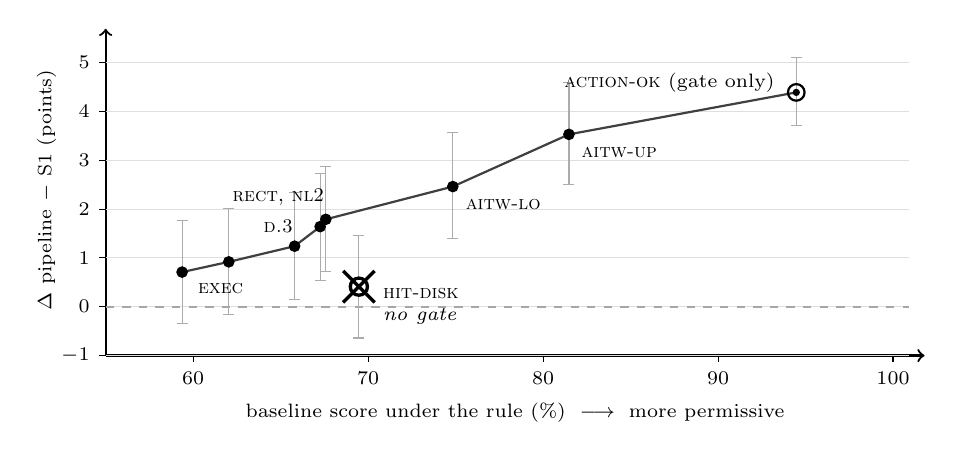
\begin{tikzpicture}[x=1cm,y=1cm]
% axes
\draw[->,thick] (0,0) -- (10.4,0);
\draw[->,thick] (0,0) -- (0,4.15);
% y grid + ticks  (y_cm = (val+1)*0.62)
\foreach \v/\c in {-1/0, 0/0.62, 1/1.24, 2/1.86, 3/2.48, 4/3.10, 5/3.72}{
  \draw[gray!25] (0,\c) -- (10.2,\c);
  \draw (0,\c) -- (-0.08,\c) node[left,font=\scriptsize] {$\v$};}
% zero line emphasised
\draw[gray!70,dashed,thick] (0,0.62) -- (10.2,0.62);
% x ticks  (x_cm = (val-55)*0.22222)
\foreach \v/\c in {60/1.111, 70/3.333, 80/5.556, 90/7.778, 100/10.0}{
  \draw (\c,0) -- (\c,-0.08) node[below,font=\scriptsize] {$\v$};}
\node[font=\scriptsize,align=center] at (5.2,-0.72)
  {baseline score under the rule (\%) $\;\longrightarrow\;$ more permissive};
\node[font=\scriptsize,rotate=90] at (-0.75,2.10) {$\Delta$ pipeline $-$ S1 (points)};
% CI bars, gated rules
\foreach \x/\lo/\hi in {0.971/0.403/1.711, 1.564/0.521/1.866, 2.400/0.707/2.071,
                        2.724/0.955/2.312, 2.796/1.066/2.400, 4.409/1.481/2.833,
                        5.884/2.176/3.466, 8.771/2.920/3.782}{
  \draw[gray!65] (\x,\lo) -- (\x,\hi);
  \draw[gray!65] (\x-0.07,\lo) -- (\x+0.07,\lo);
  \draw[gray!65] (\x-0.07,\hi) -- (\x+0.07,\hi);}
% trend through the gated rules
\draw[thick,black!75]
  (0.971,1.060) -- (1.564,1.190) -- (2.400,1.389) -- (2.724,1.637) --
  (2.796,1.730) -- (4.409,2.146) -- (5.884,2.809) -- (8.771,3.342);
% gated markers
\foreach \x/\y in {0.971/1.060, 1.564/1.190, 2.400/1.389, 2.724/1.637,
                   2.796/1.730, 4.409/2.146, 5.884/2.809}{
  \filldraw[black] (\x,\y) circle (1.9pt);}
% gate endpoint
\draw[thick] (8.771,3.342) circle (3pt);
\filldraw[black] (8.771,3.342) circle (1.1pt);
% ungated rule
\draw[gray!65] (3.216,0.223) -- (3.216,1.519);
\draw[gray!65] (3.216-0.07,0.223) -- (3.216+0.07,0.223);
\draw[gray!65] (3.216-0.07,1.519) -- (3.216+0.07,1.519);
\filldraw[white] (3.216,0.875) circle (3.1pt);
\draw[very thick] (3.216,0.875) circle (3.1pt);
\draw[very thick] (3.216-0.20,0.875-0.20) -- (3.216+0.20,0.875+0.20);
\draw[very thick] (3.216-0.20,0.875+0.20) -- (3.216+0.20,0.875-0.20);
% labels
\node[font=\scriptsize,anchor=west] at (1.05,0.85) {\rulename{exec}};
\node[font=\scriptsize,anchor=south east] at (2.50,1.44) {\rulename{d.3}};
\node[font=\scriptsize,anchor=south east] at (2.90,1.78) {\rulename{rect}, \rulename{nl2}};
\node[font=\scriptsize,anchor=north west] at (4.45,2.11) {\rulename{aitw-lo}};
\node[font=\scriptsize,anchor=north west] at (5.92,2.77) {\rulename{aitw-up}};
\node[font=\scriptsize,anchor=east] at (8.62,3.47) {\rulename{action-ok} (gate only)};
\node[font=\scriptsize,anchor=west,align=left] at (3.40,0.62)
  {\rulename{hit-disk}\\\emph{no gate}};
\end{tikzpicture}
\caption{The same comparison under every rule. Filled circles are gated coordinate rules, the
ringed point is the action gate alone, the crossed point the one rule with the gate removed; bars
are 95\% paired cluster bootstrap intervals and the dashed line is zero. The gated rules climb
smoothly toward the gate endpoint as tolerance loosens, while the ungated rule at comparable
permissiveness stays near zero. The unlabelled point is \rulename{d.3} $\wedge$ $\pm14\%$.}
\label{fig:ladder}
\end{figure}

\paragraph{Controlling for permissiveness.}
One explanation for the top of the ladder is that a permissive rule inflates all differences.
Normalisation rules this out. Dividing each $\Delta$ by that rule's own usable range from
Table~\ref{tab:cal} gives $1.1\%$ for \rulename{exec}, $1.8\%$ for \rulename{d.3}, $3.8\%$ for
\rulename{aitw-lo} and $6.5\%$ for \rulename{aitw-up}: the loosest rule has the narrowest range
and still shows the largest relative effect. The gate accounts for the pattern
instead. At \rulename{aitw-up}
the fraction of gate-passing steps that also satisfy the geometry is $86.25\%$ for the baseline
and $85.99\%$ for the pipeline, a difference that is marginally in the baseline's
favour, leaving the gate as the only component that moves.

\paragraph{Redundancy among the gated rules.}
Correlating the rules across the branches we scored, five pairs reach Pearson $\geq 0.9995$ with
Spearman exactly $1.000$, the closest being \rulename{exec} against \rulename{d.3} $\wedge$
$\pm14\%$ at $r = 0.99995$. No pair of gated rules falls below Spearman $0.976$. To the resolution of
this experiment the gated rules are one dimension observed at different tolerances, so reporting
several of them does not constitute independent evidence. Only the ungated rule stands apart:
\rulename{hit-disk} agrees with the gated ones at Spearman $0.881$ to $0.952$, the lowest
agreement anywhere in the set.

\paragraph{Invariance of the ranking.}
The coarse ordering is stable under all eight coordinate rules, where the pipeline ranks first
among the trained systems and the descriptor stage and untuned model rank last. The middle of the
table does move, however. Whether
CE2 ranks above or below the second baseline run depends on the rule. Those two are separated by
less than the run-to-run reference, so no rule is resolving anything there. Conclusions that depend only
on an ordering are therefore robust to the choice of rule, while conclusions that depend on an
effect size are not.

\paragraph{Does the spread require a gate-driven difference?}
One reading of Table~\ref{tab:ladder} is that any comparison spreads this way.
Applying the two endpoints to further pairs from the same stored predictions, the spread, by
which we mean the gate endpoint minus the geometric one, is $+3.79$ for the pair in
Table~\ref{tab:ladder} but $-0.96$ for the pipeline against CE2, the dose-matched control for its preference stage, and
$-0.38$ between the two baseline runs. Where two systems differ in localisation and not in action
type, the gate endpoint reports nothing: the pipeline beats CE2 by $+0.96$ $[+0.33,+1.62]$ on the
ungated rule and by $+0.00$ $[-0.14,+0.14]$ on the gate. The pair of endpoints therefore
separates the two channels in both directions, and the spread in Table~\ref{tab:ladder} is a
property of that comparison and not of the instrument.

%------------------------------------------------------------------------------
\section{Step-Level Attribution}
\label{sec:where}

\subsection{Conditioning on the gate}
If the pipeline improved reference rather than action formatting, it should win among steps where
both systems already pass the gate. It does not. A naive form of this test is biased, though. The
pipeline passes the gate on $98.86\%$ of steps, where the baseline passes on $94.47\%$. Conditioning on
\emph{each system's own} gate-passing set therefore adds to the pipeline's population some $4.4\%$
of steps that are, by selection, the ones the baseline had already failed. Restricting instead to the
$4{,}145$ steps ($92.9\%$) on which \emph{all} branches pass the gate removes that selection.
There, under \rulename{exec}, the baseline scores $63.15$ and the pipeline $62.03$, a
difference of $-1.12$ where the run-to-run reference is $\pm 0.36$; under the $0.14$ disc the
difference is $-0.53$ where the reference is $\pm 0.53$. These two figures are not
bootstrapped, so we read the geometric channel as flat to slightly negative without assigning it
a sign. The test is nevertheless enough to rule out an improvement on this channel.

\subsection{Partition by baseline gate status}
Partition the population by whether the baseline names the correct action type, i.e.\ by $A$
(Table~\ref{tab:slice}).
Note that its two parts reconstruct the aggregate exactly.

\begin{table}[t]
\centering
\caption{Partition by whether the S1 baseline names the correct action type ($A$), scored with
\rulename{exec}.
The baseline scores zero on the first slice by construction, since \rulename{exec} contains
$A$; the informative quantities are how much the pipeline recovers there and what it costs
elsewhere. We define the partition by the baseline's behaviour alone, so it is not chosen after
seeing the pipeline. Repeating the analysis against the second baseline run reproduces it.}
\label{tab:slice}
\small
\begin{tabular}{lrrrrr}
\toprule
slice & steps & share & S1\,101 & pipeline & $\Delta$\\
\midrule
S1 fails $A$      & \phantom{0,}252 & \phantom{0}5.65\% & \phantom{0}0.00 &
34.92 & $+34.92$\\
S1 passes $A$     & 4{,}211 & 94.35\% & 62.65 & 61.58 & $-1.07$\\
\midrule
whole population              & 4{,}463 & 100\% & 59.11 & 60.07 & $+0.96$\\
\midrule
\multicolumn{6}{l}{\emph{same analysis against the second baseline run:}}\\
\multicolumn{6}{l}{\quad slice $5.42\%$, $\Delta +36.36$; complement $\Delta -1.61$}\\
\bottomrule
\end{tabular}
\end{table}

Far from being spread across the population, the effect is concentrated. On the slice where the baseline names the
wrong kind of action, the pipeline recovers about a third of the steps from a floor of zero; on
the $94\%$ where the action was already correct, it is marginally worse. Each half replicates
against the second baseline run, so neither is an artefact of a single training run.

\subsection{A control for the per-sentence win rate}
Aggregate differences do not show how an improvement is distributed. We compared the
two systems sentence by sentence. On $46.0\%$ of steps the pipeline emits the baseline's sentence up to case and punctuation,
with $\Delta = -0.24$ there, since punctuation alone occasionally moves the listener. Nearly all
movement lies inside the $2{,}409$ steps whose
wording changed, where the pipeline saves $329$ and breaks $281$, a net of $48$ steps, or $+1.08$
points overall.

To calibrate a net win rate of $1.99\%$ per changed sentence, we ran the same ledger between the
two baseline runs, which differ only in initialisation. That comparison changes $33.1\%$ of the
sentences and wins $154$ and loses $129$, a net rate of $1.69\%$. Per changed sentence, the
pipeline's net advantage is therefore close to what training variation alone
produces, and accumulates further only because more sentences are rewritten. The action channel
behaves differently, since among changed sentences the gate improves by $+8.30$ points, with no
comparable movement in the control. This test separates the two channels, and on this evidence only
one of them carries a signal.

\subsection{Action-type distribution}
\label{sec:mech}
The action-type distribution identifies the mechanism directly (Table~\ref{tab:verbs}). Every
scored step is a touch, so a sentence led by \emph{scroll}, \emph{swipe} or \emph{type} scores
zero regardless of how well it names the target. Counted anywhere in the sentence and not
only at the start, $6.88\%$ of baseline sentences contain a non-touch verb, compared with $0.56\%$ for
the pipeline and $0.29\%$ for human references.

\begin{table}[t]
\centering
\caption{Leading verb of the generated sentence, with two descriptive statistics, over the
$4{,}463$ scored steps. Every gold action is a touch, so \emph{scroll}, \emph{swipe} and
\emph{type} are always incorrect. ``unique'' is the share of distinct lowercased sentences.}
\label{tab:verbs}
\small
\begin{tabular}{lrrrrrrr}
\toprule
& \multicolumn{5}{c}{leading verb} & &\\
\cmidrule(lr){2-6}
branch & \emph{scroll} & \emph{swipe} & \emph{type} & \emph{click} & \emph{select}
& words/sent. & unique\\
\midrule
untuned model     & \phantom{0}0 & \phantom{0}28 & 66 & 3{,}736 & \phantom{0}11 & 13.98 &
91.7\%\\
S1 baseline       & 33 & 140 & 54 & 3{,}543 & 222 & \phantom{0}7.83 & 64.6\%\\
full pipeline     & \phantom{0}0 & \phantom{0}11 & \phantom{0}3 & 3{,}895 & 176 &
\phantom{0}8.10 & 67.0\%\\
human reference   & \phantom{0}0 & \phantom{00}1 & \phantom{0}6 & 3{,}599 & 252 &
\phantom{0}7.80 & 75.5\%\\
\bottomrule
\end{tabular}
\end{table}

Two observations qualify this. First, the untuned model already passes the action gate on
$96.46\%$ of steps, \emph{above} the baseline's $94.47\%$. Supervised fine-tuning therefore
appears to introduce the verb confusion. Our later stages are largely repairing an earlier stage
of the same pipeline, not adding a capability the base model lacked. Why fine-tuning introduces it is
not something these experiments settle, since the supervised targets are human instructions of the
same kind, and those name a non-touch action on only $0.29\%$ of scored steps. Second, the
correction is
specific to this population. Because every scored step is a touch, collapsing toward \emph{click
on\ldots} is nearly costless here, and the pipeline does collapse in that direction. On a
realistic action mix it would likely cost something. We therefore characterise the contribution as improved
action-type consistency rather than improved element reference.

%------------------------------------------------------------------------------
\section{Cross-Checks}
\label{sec:cross}

\subsection{A second listener}
A single model listener may be exploitable. We therefore rescored every branch with
Phi-4-multimodal~\cite{phi4}, which is not built on Qwen and was not trained on AndroidControl.
Its protocol also differs by design, since clickable elements are numbered on the image and the
listener selects a number, a multiple choice instead of a coordinate regression. It scores human
references at $54.94$, the pipeline at $45.78$, the baseline at $44.63$, contentless text at
$15.86$ and random guessing at $10.06$. The ordering is preserved, with a margin of $+1.14$ and a
95\% interval of $[+0.23,+2.10]$. Its ceiling is well below UGround's, so we use it as a check
and not for headline numbers. Agreement between the two listeners is modest ($\kappa$ from $0.25$ to
$0.44$ by branch). We read that as evidence that they fail on different steps, which makes the
preserved ordering harder to explain as an artefact of either one.

\subsection{Reference-overlap metrics}
We also scored the standard text metrics against the reference instruction. They split into two
groups: the baseline leads on BLEU-4, CIDEr-D and SPICE, the pipeline on METEOR, ROUGE-L and
BERTScore. A natural explanation is that surface-overlap metrics penalise
paraphrase while soft-matching ones tolerate it, but two findings contradict that. SPICE is the
most semantic metric in the set, and the pipeline loses on it. The ROUGE-L lead is a length
effect: over the $2{,}631$ steps ($59\%$) on which the two systems emit sentences of equal word
count it reverses, from $68.47$ against $67.27$ to $74.66$ against $75.00$.

Recall the partition of Sect.~\ref{sec:where}, which BLEU-4 exhibits directly.
Overall the baseline leads, $51.80$ to $50.18$. On the $252$ steps where it misses the action
gate the pipeline rises from $10.26$ to $36.81$; on the $4{,}211$ where the verb was
already correct it rewards adequate sentences and loses ground, $53.68$ to $50.91$. That second
slice is sixteen times larger and so sets the sign of the aggregate, whereas the execution score is bounded at each step
and is set by the first. The two families seem to report the same underlying event under different
weightings, which is the pattern Yu et al.~\cite{yu2016} describe and a reason to read reference
overlap alongside execution and not in place of it.

%------------------------------------------------------------------------------
\section{Discussion}
\label{sec:disc}

A paper reporting execution-based scores for GUI instruction generation should give four things.
First, the rule it used, written out as a predicate rather than cited by name. Second, the same
comparison under at least one rule with the action gate removed. Third, the ceiling its own
instrument assigns to human reference sentences. Fourth, at least one shortcut floor. Note that the last three require no additional training or inference, being
recomputed from stored predictions.

Adopting the strictest available rule is not an adequate substitute, because strictness is not
the relevant axis. \rulename{d.3} is stricter than \rulename{aitw-up} and is still multiplied by the
same gate, so adopting it lowers every number without separating the two channels. Separation
requires reporting the gate and an ungated rule next to the gated score, which is what agent
papers already do when they list action type and grounding beside step success~\cite{osatlas}.
We are asking instruction generation to adopt the same habit.

We can apply the same decomposition inside the system under test. All three stages intervene on a
declaration slot that the listener never sees, and parsing the point the model declares for
itself splits the task into choosing an element and then describing it. Our
descriptor stage chooses correctly on $71.10\%$ of steps, the preference stage on $70.23\%$, the
full pipeline on $71.82\%$; where the choice is correct, the sentence is executable $82.05\%$,
$82.31\%$ and $81.43\%$ of the time. Between the descriptor stage and the full pipeline neither quantity moves by more than a point,
while the aggregate rises from $57.18$ to $60.07$, reproducing the gate result from inside the model. Both
element selection and phrasing remain well short of saturation.

%------------------------------------------------------------------------------
\section{Limitations and Future Work}
\label{sec:limits}

Our study covers one dataset, Android touch steps from AndroidControl, and uses UGround as the
primary listener. AndroidControl does not ship the annotation boxes that \rulename{d.3} and
\rulename{aitw-lo} assume, so we take the smallest accessibility node containing the recorded
touch, which may make those two rules somewhat stricter than the originals. Extending the ladder
to web and desktop interfaces, to non-touch actions and to further listeners is a natural next
step.

%------------------------------------------------------------------------------
\section{Conclusion}

Execution-based scoring remains the appropriate instrument for GUI instruction generation. Its
current use, however, understates how much depends on the matching rule. Because the rules in circulation all
multiply a geometric test by the same action-type gate, a single comparison can be reported as
$+0.41$ or as $+4.39$ depending only on which rule its authors chose. At the step level, the
whole effect sits in the $5.65\%$ of steps where the baseline names the wrong action type, and the
geometric channel is flat once the gate is held fixed. We recommend reporting both endpoints
alongside the gated score, together with a ceiling and a floor.

%------------------------------------------------------------------------------
\begin{thebibliography}{99}

\bibitem{androidcontrol}
Li, W., Bishop, W.E., Li, A., Rawles, C., Campbell-Ajala, F., Tyamagundlu, D., Riva, O.:
On the effects of data scale on UI control agents. In: Advances in Neural Information Processing
Systems 37, Datasets and Benchmarks Track (2024)

\bibitem{aitw}
Rawles, C., Li, A., Rodriguez, D., Riva, O., Lillicrap, T.: Android in the Wild: a large-scale
dataset for Android device control. In: Advances in Neural Information Processing Systems 36,
Datasets and Benchmarks Track (2023)

\bibitem{uground}
Gou, B., Wang, R., Zheng, B., Xie, Y., Chang, C., Shu, Y., Sun, H., Su, Y.: Navigating the
digital world as humans do: universal visual grounding for GUI agents. In: International
Conference on Learning Representations (2025)

\bibitem{seeclick}
Cheng, K., Sun, Q., Chu, Y., Xu, F., Li, Y., Zhang, J., Wu, Z.: SeeClick: harnessing GUI
grounding for advanced visual GUI agents. In: Proceedings of the 62nd Annual Meeting of the
Association for Computational Linguistics (2024)

\bibitem{osatlas}
Wu, Z., Wu, Z., Xu, F., Wang, Y., Sun, Q., Jia, C., Cheng, K., Ding, Z., Chen, L.,
Liang, P.P., Qiao, Y.: OS-ATLAS: a foundation action model for generalist GUI agents. In:
International Conference on Learning Representations (2025)

\bibitem{mind2web}
Deng, X., Gu, Y., Zheng, B., Chen, S., Stevens, S., Wang, B., Sun, H., Su, Y.: Mind2Web: towards
a generalist agent for the web. In: Advances in Neural Information Processing Systems 36,
Datasets and Benchmarks Track (2023)

\bibitem{widgetcap}
Li, Y., Li, G., He, L., Zheng, J., Li, H., Guan, Z.: Widget captioning: generating natural
language description for mobile user interface elements. In: Proceedings of the 2020 Conference
on Empirical Methods in Natural Language Processing (2020)

\bibitem{mao2016}
Mao, J., Huang, J., Toshev, A., Camburu, O., Yuille, A., Murphy, K.: Generation and comprehension
of unambiguous object descriptions. In: IEEE Conference on Computer Vision and Pattern
Recognition (2016)

\bibitem{yu2016}
Yu, L., Poirson, P., Yang, S., Berg, A.C., Berg, T.L.: Modeling context in referring expressions.
In: European Conference on Computer Vision (2016)

\bibitem{luo2017}
Luo, R., Shakhnarovich, G.: Comprehension-guided referring expressions. In: IEEE Conference on
Computer Vision and Pattern Recognition (2017)

\bibitem{disclip}
Bracha, L., Shaar, E., Shamsian, A., Fetaya, E., Chechik, G.: DisCLIP: open-vocabulary referring expression generation.
In: British Machine Vision Conference (2023)

\bibitem{newman2020}
Newman, B., Cohn-Gordon, R., Potts, C.: Communication-based evaluation for natural language
generation. In: Proceedings of the Society for Computation in Linguistics (2020)

\bibitem{zhao2021}
Zhao, M., Anderson, P., Jain, V., Wang, S., Ku, A., Baldridge, J., Ie, E.: On the evaluation of
vision-and-language navigation instructions. In: Proceedings of the 16th Conference of the
European Chapter of the Association for Computational Linguistics (2021)

\bibitem{refoi}
Ma, Z., et al.: Vision language models are not pragmatically competent in referring expression
generation. arXiv:2504.16060 (2025), preprint

\bibitem{reimers2017}
Reimers, N., Gurevych, I.: Reporting score distributions makes a difference: performance study of
LSTM-networks for sequence tagging. In: Proceedings of the 2017 Conference on Empirical Methods
in Natural Language Processing (2017)

\bibitem{cameron2008}
Cameron, A.C., Gelbach, J.B., Miller, D.L.: Bootstrap-based improvements for inference with
clustered errors. Review of Economics and Statistics \textbf{90}(3), 414--427 (2008)

\bibitem{qwen25vl}
Bai, S., et al.: Qwen2.5-VL technical report. arXiv:2502.13923 (2025), preprint

\bibitem{lora}
Hu, E.J., Shen, Y., Wallis, P., Allen-Zhu, Z., Li, Y., Wang, S., Wang, L., Chen, W.: LoRA:
low-rank adaptation of large language models. In: International Conference on Learning
Representations (2022)

\bibitem{qlora}
Dettmers, T., Pagnoni, A., Holtzman, A., Zettlemoyer, L.: QLoRA: efficient finetuning of
quantized LLMs. In: Advances in Neural Information Processing Systems 36 (2023)

\bibitem{orpo}
Hong, J., Lee, N., Thorne, J.: ORPO: monolithic preference optimization without reference model.
In: Proceedings of the 2024 Conference on Empirical Methods in Natural Language Processing (2024)

\bibitem{grpo}
Shao, Z., Wang, P., Zhu, Q., Xu, R., Song, J., Bi, X., Zhang, H., Zhang, M., Li, Y.K., Wu, Y.,
Guo, D.: DeepSeekMath: pushing the limits of mathematical reasoning in open language models.
arXiv:2402.03300 (2024), preprint

\bibitem{llamafactory}
Zheng, Y., Zhang, R., Zhang, J., Ye, Y., Luo, Z., Feng, Z., Ma, Y.: LlamaFactory: unified
efficient fine-tuning of 100+ language models. In: Proceedings of the 62nd Annual Meeting of the
Association for Computational Linguistics, System Demonstrations (2024)

\bibitem{phi4}
Abouelenin, A., et al.: Phi-4-Mini technical report: compact yet powerful multimodal language
models via mixture-of-LoRAs. arXiv:2503.01743 (2025), preprint

\end{thebibliography}

\end{document}
